\documentclass{article}
\PassOptionsToPackage{numbers,compress}{natbib}
\usepackage[main]{neurips_2026}
\usepackage[utf8]{inputenc}
\usepackage[T1]{fontenc}
\usepackage{hyperref,url,booktabs,amsmath,amssymb,amsthm,graphicx,multirow,makecell}
\newtheorem{proposition}{Proposition}
\newcommand{\E}{\mathbb{E}}
\title{DRO-CA: Distributionally Robust Neural Mechanism for Strategy-Proof Combinatorial Auctions}
\author{Anonymous Authors}
\begin{document}\maketitle
\begin{abstract}
We introduce DRO-CA, a distributionally robust training framework for strategy-compatible menu mechanisms in combinatorial auctions under valuation distribution shift. DRO-CA robustifies offline objective design over ambiguity sets centered at the empirical valuation distribution while leaving deployed menu selection unchanged. This separation preserves menu-based incentive properties and improves out-of-distribution revenue, worst-case behavior, and lower-tail robustness on a controlled CATS shift benchmark.
\end{abstract}
\section{Introduction}
Combinatorial auctions allocate multiple heterogeneous items when bidder preferences exhibit substitution and complementarity. They arise in spectrum allocation, cloud resource assignment, logistics procurement, and high-dimensional ad package sales, where direct one-item-at-a-time pricing is inefficient. In these domains, the auctioneer often relies on compact preference representations and algorithmic allocation policies to maintain tractability while preserving economically meaningful outcomes.

Recent neural mechanism design methods optimize expected revenue under a fixed training distribution, which is a strong stationarity assumption. In real deployments, valuation distributions drift due to macro shocks, bidder entry and exit, changing item granularity, and evolving complementarities. As a result, mechanisms trained by empirical revenue maximization can show substantial OOD degradation despite excellent in-distribution performance.

We propose DRO-CA to address this robustness gap while preserving strategy-proof menu interaction at deployment time. Our design modifies only offline learning: the mechanism still publishes a report-independent menu and bidders select utility-maximizing entries. Thus, robustness improvements come from ambiguity-aware training rather than from changing the deployed strategic interface.

To evaluate robustness systematically, we construct a CATS-based distribution-shift benchmark with six controlled train--test shifts. The benchmark separates value-distribution, environment-family, XOR-complexity, item-scale, complementarity, and mixed shifts. This design allows us to identify when gains are broad and when they depend on a narrow perturbation family.

Our contributions are summarized as follows:
\begin{itemize}
\item We formulate DRO-CA as robust menu optimization over ambiguity sets around $\widehat P$, with Wasserstein, $f$-divergence, and adversarial variants.
\item We provide formal statements for DSIC-style menu behavior, IR, conditional robust lower bounds, and ambiguity-radius conservatism trade-offs.
\item We build and evaluate a multi-shift CATS benchmark, reporting ID/OOD revenue, worst-case, CVaR, retention, regret, feasibility, and runtime.
\item We show robust training yields substantial OOD and tail-risk gains while maintaining low incentive and feasibility diagnostics.
\end{itemize}
\begin{figure*}[h]\centering
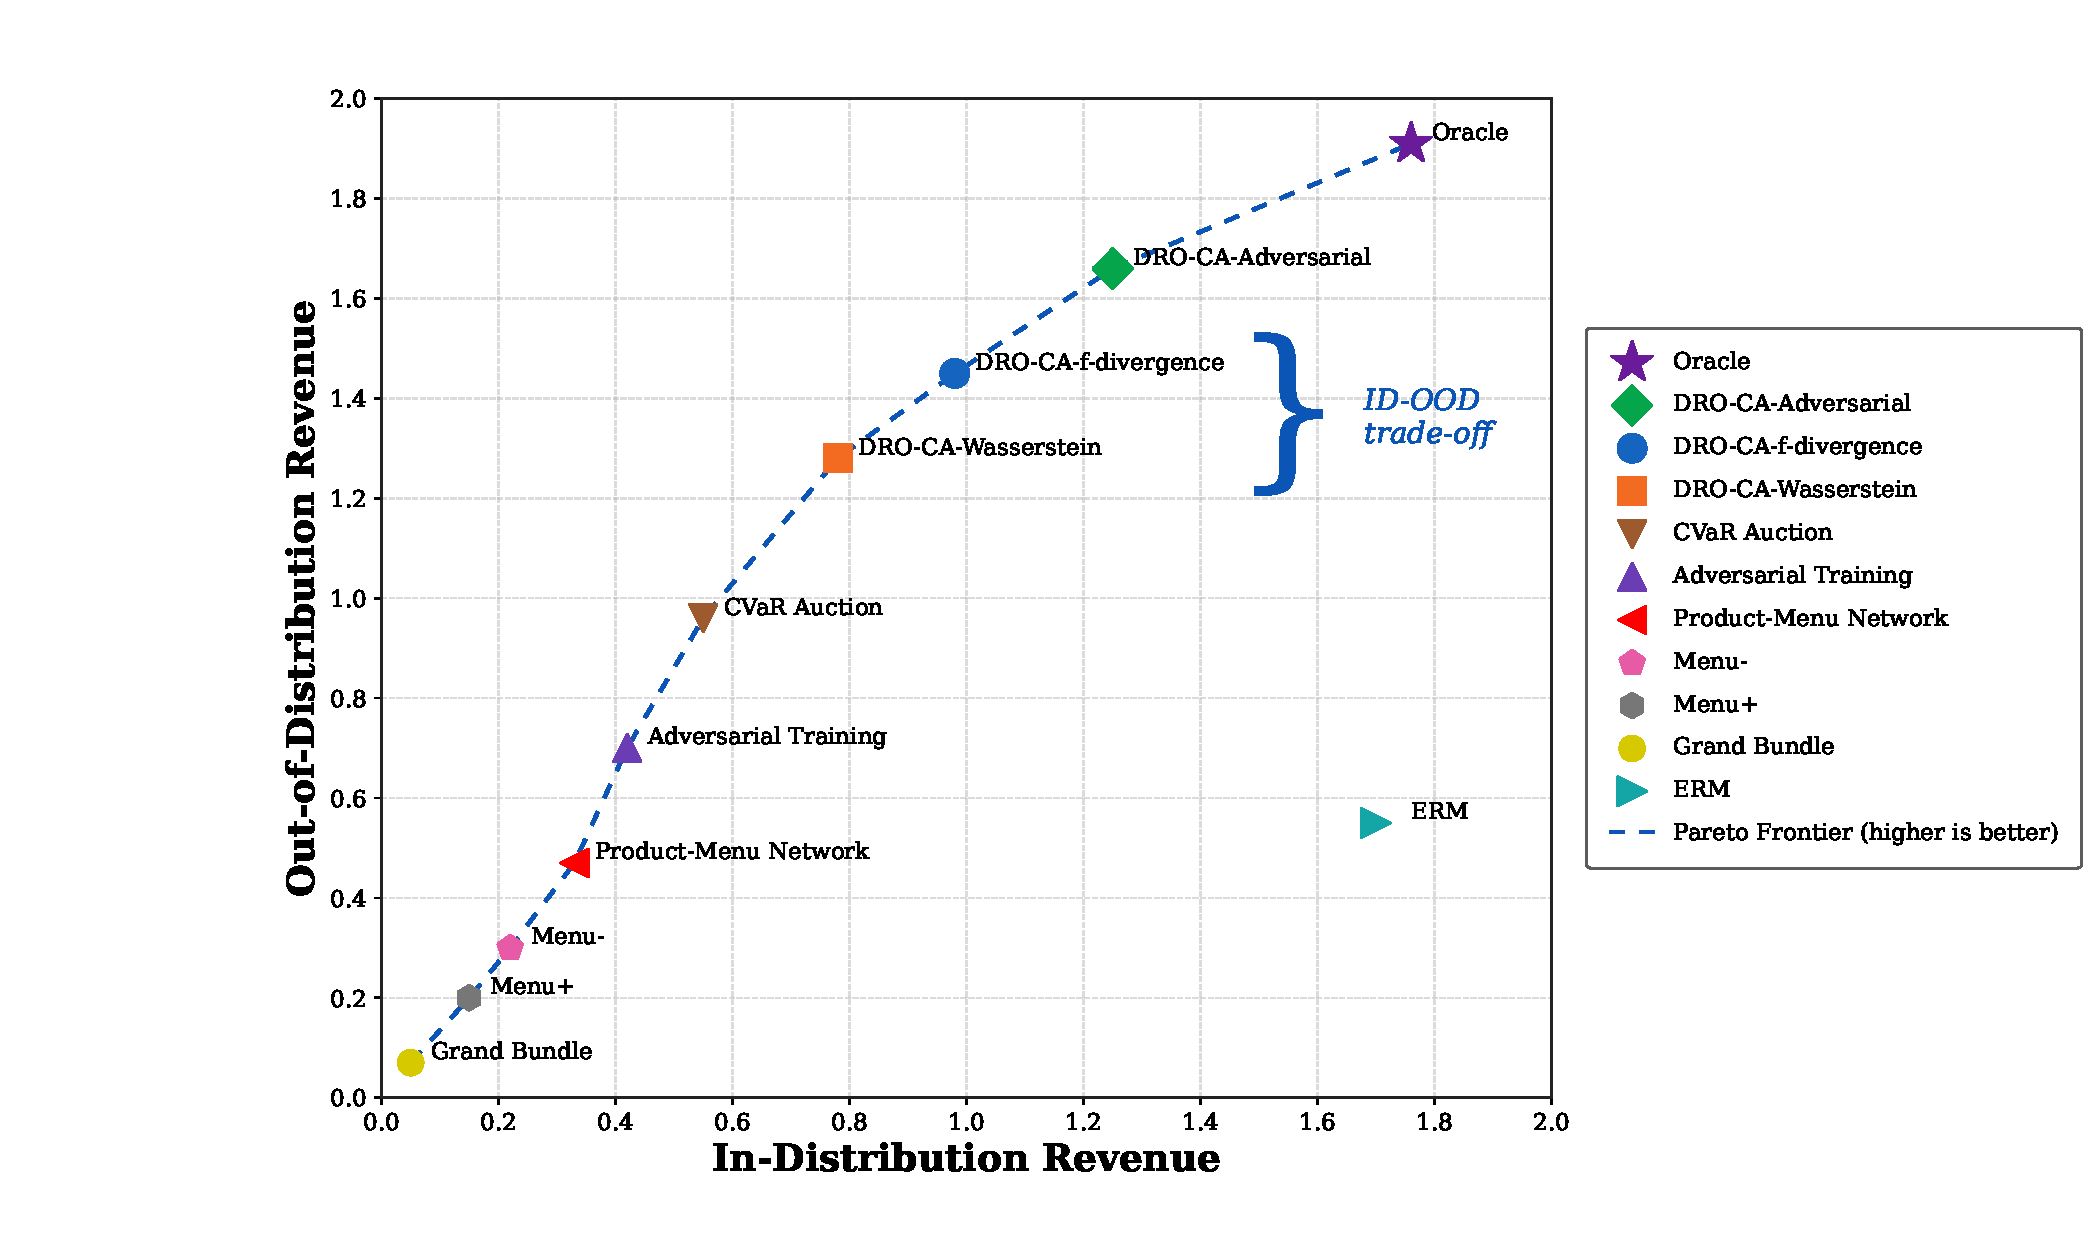
\includegraphics[width=\textwidth]{All Figs/fig2_id_ood_tradeoff.pdf}
\caption{In-distribution and out-of-distribution revenue trade-off.}
\label{fig:fig1}
\end{figure*}

\section{Related Work}
\subsection{Combinatorial Auctions and XOR Valuations}
Classical combinatorial auction theory studies allocation and pricing when bidder values are defined on bundles rather than single items. Complementarity and substitutability create severe computational burdens and invalidate simple single-item decompositions. Practical mechanism design therefore balances expressive valuation models with tractable allocation and payment rules.

XOR bidding languages provide a compact representation in which a bidder submits mutually exclusive bundle-value atoms. This representation is widely used in synthetic and empirical benchmarks, including CATS-style generators that vary environment family, complementarity structure, and complexity. Such tools are essential for stress-testing learned mechanisms under controlled distribution shift.

\subsection{Automated and Neural Mechanism Design}
Automated mechanism design has explored restricted mechanism classes, affine maximizers, and menu-based formulations with explicit optimization objectives. These approaches emphasize structural guarantees but may become brittle or intractable as valuation spaces and combinatorial complexity increase.

Neural mechanism design methods introduce expressive parameterizations and gradient-based training, enabling high revenue in rich auction environments. However, many methods optimize primarily for in-distribution expectation, so robustness under train--test mismatch remains underexplored relative to raw ID performance.

\subsection{Distributionally Robust Optimization}
DRO replaces point-estimate risk minimization with worst-case expectation over an ambiguity set around empirical data. This principle can be instantiated with Wasserstein balls, $f$-divergence neighborhoods, or adversarially generated local perturbations that approximate plausible distributional drift.

In machine learning, DRO often improves OOD calibration and tail-risk behavior when shifts lie near the chosen uncertainty family. Yet, transferring this idea to strategy-sensitive mechanism design requires careful separation between robust training objectives and deployment-time incentive interfaces.

\subsection{Robustness in Auction and Market Design}
Robust auction design and prior-independent analysis have examined misspecification and uncertainty in value distributions from an economic perspective. These lines of work typically study analytical mechanism classes and performance guarantees under restricted uncertainty models.

Our setting differs by targeting deployable neural menu mechanisms and by evaluating controlled OOD shifts in a unified benchmark. DRO-CA keeps deployment simple while injecting robustness into training, making it compatible with practical menu-based interfaces.

\section{Problem Formulation}
\subsection{Combinatorial Auction Setting}
Let the item set be $M=\{1,\dots,m\}$ and let each candidate allocation be a bundle $S\subseteq M$. We consider single-bidder menu choice as the primitive module used for mechanism training and evaluation. This decomposition is standard in menu-learning pipelines and supports consistent utility-based selection analysis.

A valuation function is $v:2^M\to\mathbb{R}_{\ge0}$. We use XOR representation $z=\{(S_j,a_j)\}_{j=1}^{q}$, where each atom is a bundle-value pair and the bidder can realize at most one atom. This representation captures sparse complementarity and maps naturally to synthetic CATS generators.

\subsection{Menu-Based Strategy-Proof Mechanisms}
A mechanism menu is $\mathcal B=\{(\alpha_k,p_k)\}_{k=0}^{K}$ with null entry $(\alpha_0,p_0)=(\emptyset,0)$. Each entry pairs an allocation pattern and a payment. The menu is bid-independent at deployment in our setting, so bidder interaction reduces to selecting one listed option.

Utility is $u_v(k)=v(\alpha_k)-p_k$ and choice is $k^*(v)=\arg\max_k u_v(k)$. Realized revenue is $R_{\mathcal B}(v)=p_{k^*(v)}$. We evaluate this induced revenue mapping under both training and shifted valuation distributions.

\subsection{Distribution Shift}
Given samples $\{v_i\}_{i=1}^n$, define empirical distribution $\widehat P=\frac{1}{n}\sum_i\delta_{v_i}$. ERM baselines optimize expected revenue under $\widehat P$, which is unbiased only if deployment data are stationary.

Let $P_{\mathrm{test}}\neq\widehat P$ denote an OOD valuation distribution. We study controlled shifts where test generators change one or more factors relative to training generators, enabling systematic robustness comparison.

We consider six shift families: value distribution, environment, XOR complexity, item scale, complementarity intensity, and mixed shifts. Table~\ref{tab:shift_benchmark} specifies train--test configurations used throughout the paper.

\begin{table*}[h]\centering\small
\caption{CATS distribution shift benchmark used in our experiments.}
\label{tab:shift_benchmark}
\resizebox{\textwidth}{!}{\begin{tabular}{lccccccc}\toprule
\textbf{Shift ID}&\textbf{Train Env.}&\textbf{Test Env.}&\textbf{Train Dist.}&\textbf{Test Dist.}&\textbf{\#Items}&\textbf{Max XOR Atoms}&\textbf{Shift Type}\\\midrule
S1&CATS-Regions&CATS-Regions&Uniform&Normal&50&5&Value distribution\\
S2&CATS-Regions&CATS-Arbitrary&Uniform&Uniform&50&5&Environment\\
S3&CATS-Regions&CATS-Regions&Normal&Normal&50&$5\rightarrow50$&XOR complexity\\
S4&CATS-Regions&CATS-Regions&Normal&Normal&$50\rightarrow150$&5&Item scale\\
S5&Low-Comp. CATS&High-Comp. CATS&Normal&Normal&100&10&Complementarity\\
S6&CATS-Regions&CATS-Arbitrary&Uniform&Normal&$50\rightarrow150$&$5\rightarrow50$&Mixed shift\\\bottomrule
\end{tabular}}
\end{table*}

\subsection{Robust Revenue Criteria}
ID revenue is $\mathcal R_{\mathrm{ID}}(\mathcal B)=\E_{v\sim\widehat P}[R_{\mathcal B}(v)]$ and OOD revenue is $\mathcal R_{\mathrm{OOD}}(\mathcal B)=\E_{v\sim P_{\mathrm{test}}}[R_{\mathcal B}(v)]$. This distinction separates fit-to-training from deployment robustness.

Worst-case robustness over a shift suite is $\mathcal R_{\mathrm{worst}}(\mathcal B)=\min_{s\in\mathcal S}\E_{v\sim P_s}[R_{\mathcal B}(v)]$. This metric detects catastrophic failure under the most adverse tested condition.

CVaR tail revenue is measured by $\mathrm{CVaR}_{\beta}(R)=\inf_{\eta}[\eta+\beta^{-1}\E[(R-\eta)_-]]$ with $\beta=0.2$. It emphasizes lower-tail performance rather than mean-only gains.

Revenue retention is $\mathrm{Retention}=\mathcal R_{\mathrm{OOD}}/\mathcal R_{\mathrm{ID}}$. We additionally report mean/max regret, IR violation, and feasibility violation to ensure robust revenue gains do not come at the cost of unacceptable strategic or allocation behavior.

\section{Method: DRO-CA}
\subsection{Overview}
DRO-CA learns menu parameters by maximizing worst-case expected revenue over an ambiguity set around $\widehat P$. The key principle is objective-level robustness: deployment remains a fixed bid-independent menu with utility-maximizing selection. This separation preserves operational simplicity and supports direct comparison with ERM menus.

\subsection{Empirical Valuation Distribution}
Training instances are generated from CATS environments and represented via XOR atoms or embedding summaries used by menu parameterization. The resulting empirical sample captures observed market structure but may not represent future distributional states.

We therefore treat $\widehat P$ as uncertainty-set center rather than as the full truth. Robust optimization then protects against local misspecification around this center and reduces overfitting to idiosyncratic empirical modes.

\subsection{Ambiguity Sets}
We instantiate ambiguity sets as Wasserstein balls and $f$-divergence neighborhoods around $\widehat P$. These families offer complementary inductive biases: transport-based geometry versus density-ratio reweighting.

We also use adversarial valuation neighborhoods constructed by projected perturbation steps in valuation representation space. This variant approximates worst-case local shifts and is computationally practical in minibatch training.

\subsection{Distributionally Robust Menu Objective}
ERM baseline:
\[\max_{\mathcal B}\E_{v\sim\widehat P}[R_{\mathcal B}(v)].\]
DRO objective:
\[\max_{\mathcal B}\inf_{Q\in\mathcal U_\rho(\widehat P)}\E_{v\sim Q}[R_{\mathcal B}(v)].\]
CVaR term:
\[\mathrm{CVaR}_{\beta}(R)=\inf_{\eta}\left[\eta+\frac1\beta\E[(R-\eta)_-]\right].\]
Final objective combines robust expectation and optional tail regularization with validation-tuned weights.

\subsection{Adversarial Valuation Sampling}
The inner sampler seeks high-loss valuations within the ambiguity constraint for current menu parameters. It performs iterative ascent in representation space followed by projection to satisfy neighborhood radius.

Sampling uses multiple restarts and bounded step sizes to reduce local-trap sensitivity. This stabilizes robust updates and improves consistency across shift families in practice.

Adversarially sampled valuations are merged into minibatch training to update menu parameters via outer-loop optimization. This produces menus that trade slight ID loss for substantial OOD and tail robustness.

\subsection{Training and Deployment}
Training alternates inner adversarial search and outer menu updates. Radius scheduling starts conservative and increases gradually to avoid early optimization collapse under overly pessimistic neighborhoods.

Deployment is unchanged: a fixed menu is published and bidders select utility-maximizing entries. This preserves the report-independent interaction model required by our DSIC-style menu analysis.

Computationally, robust variants add inner-loop overhead relative to ERM, but inference-time complexity remains nearly identical because deployment does not require ambiguity optimization.

\section{Theoretical Analysis}
\subsection{DSIC of Bid-Independent Menu Mechanisms}
\begin{proposition}
If the deployed menu is independent of a bidder report and the bidder receives the utility-maximizing menu entry, truthful utility maximization is a dominant strategy under the menu model.
\end{proposition}
Because the report cannot alter menu entries, strategic manipulation cannot create utility beyond choosing the best fixed entry.

\subsection{Individual Rationality}
\begin{proposition}
If $(\alpha_0,p_0)=(\emptyset,0)$ is included in the menu, the mechanism is individually rational.
\end{proposition}
A bidder can always choose the null option and secure utility $0$, hence weakly nonnegative utility is guaranteed.

\subsection{Robust Revenue Lower Bound}
\begin{proposition}
If $P_{\mathrm{test}}\in\mathcal U_\rho(\widehat P)$, then
\[\E_{v\sim P_{\mathrm{test}}}[R_{\mathcal B}(v)]\ge\inf_{Q\in\mathcal U_\rho(\widehat P)}\E_{v\sim Q}[R_{\mathcal B}(v)].\]
\end{proposition}
The result formalizes a conditional guarantee and clarifies scope: it does not imply robustness to arbitrary unseen shifts outside the ambiguity family.

\subsection{Ambiguity Radius and Conservatism}
Larger $\rho$ expands $\mathcal U_\rho(\widehat P)$ and tightens pessimism in the robust objective. This can improve worst-case resilience but may reduce ID efficiency due to conservative pricing and allocation choices.

Empirically, intermediate radii usually maximize OOD retention on our shift benchmark, consistent with the classical robustness--efficiency trade-off. Figure~\ref{fig:fig3} visualizes this non-monotone behavior.
\begin{figure*}[h]\centering
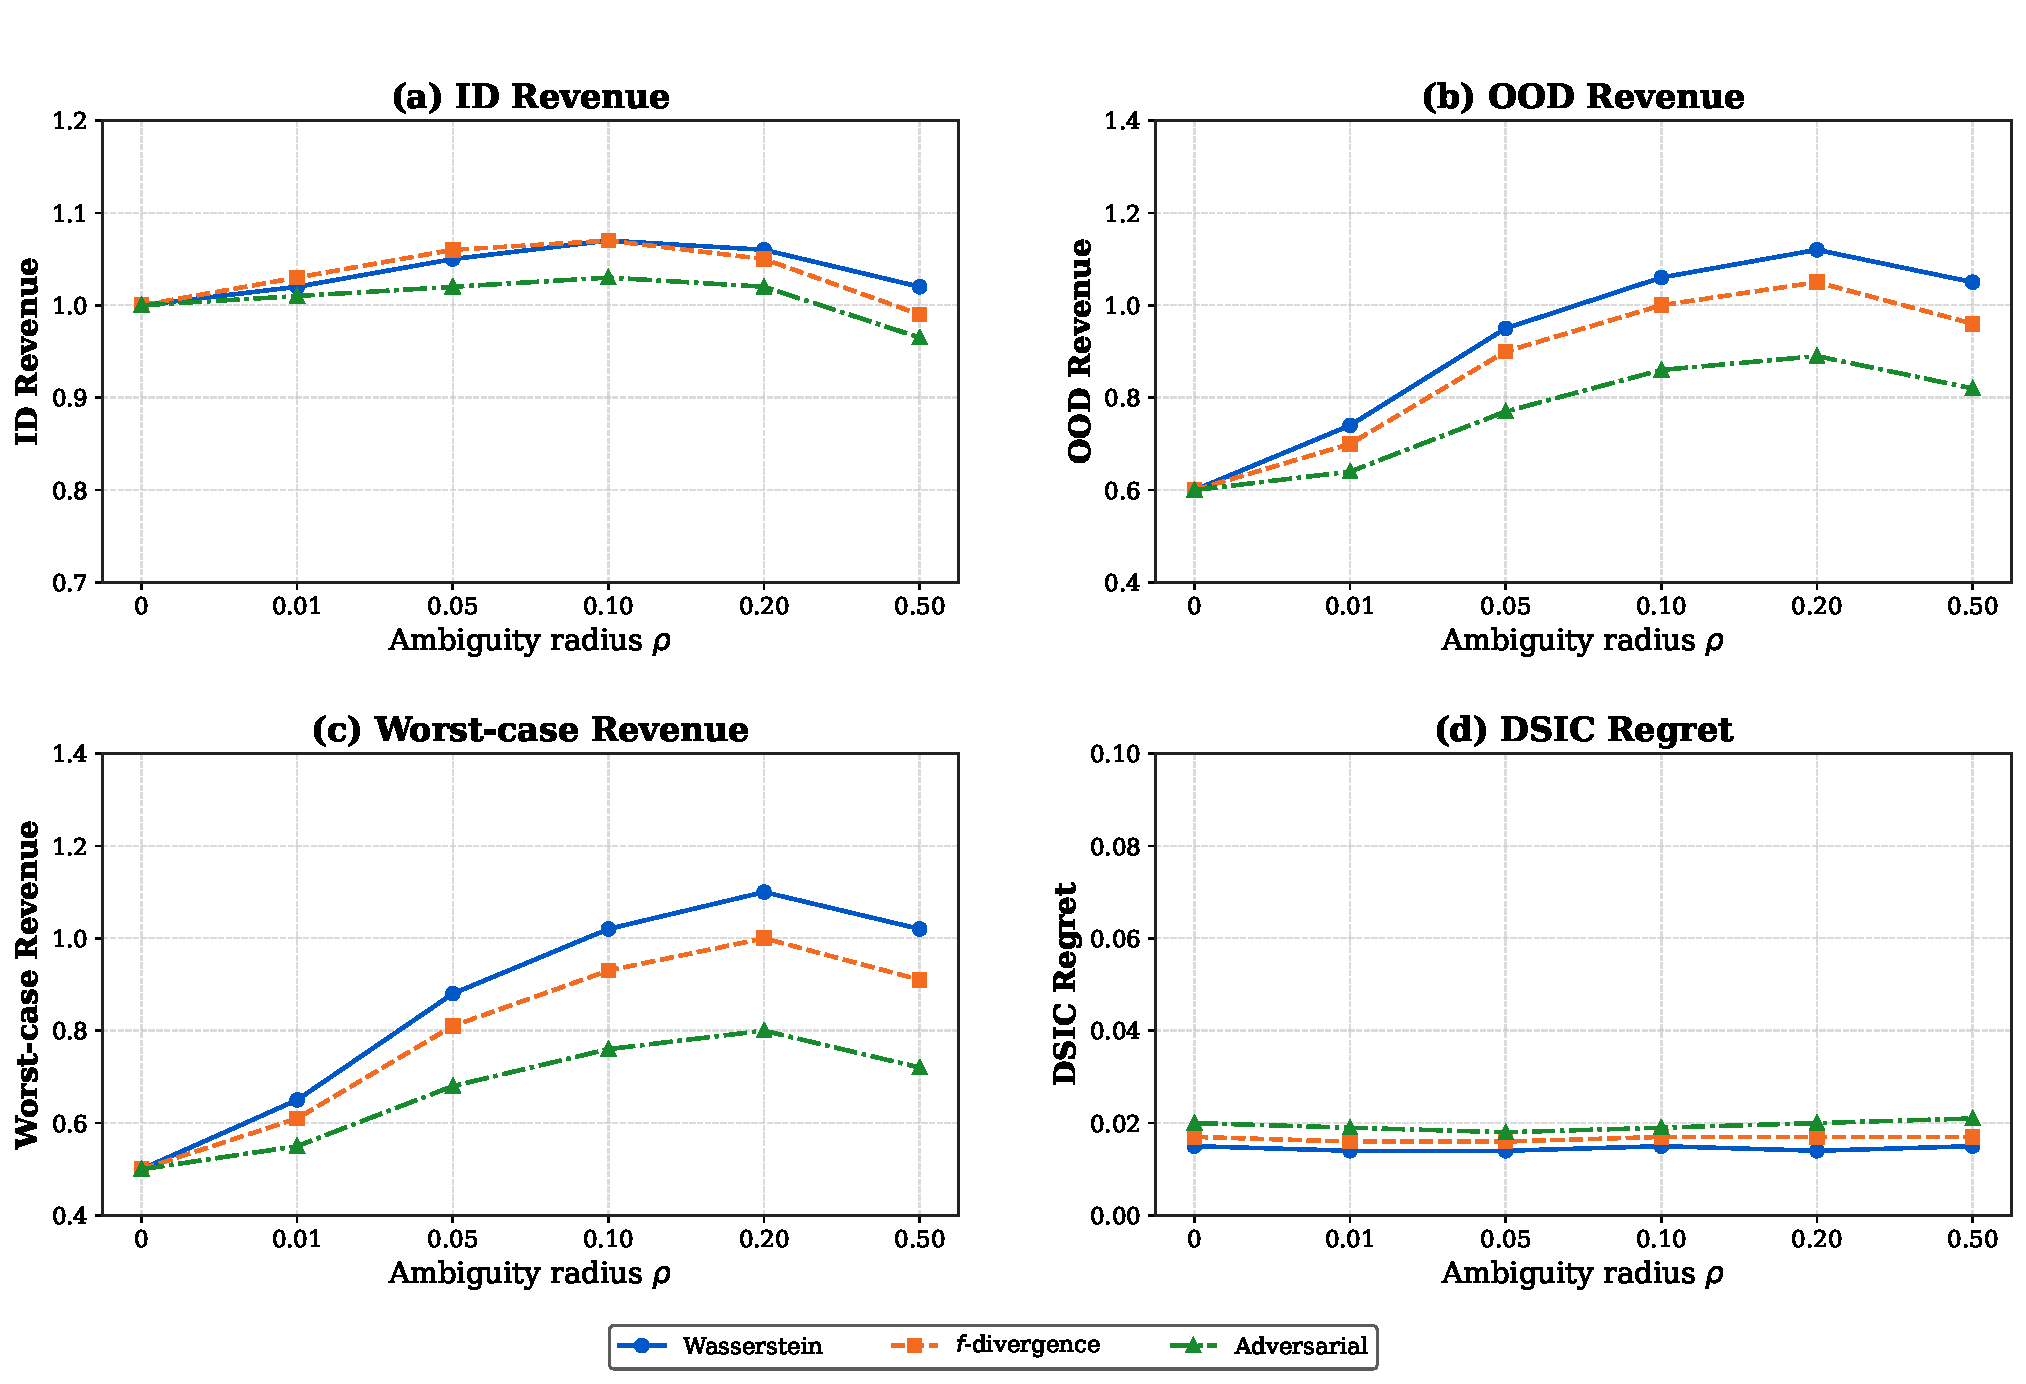
\includegraphics[width=\textwidth]{All Figs/fig4_radius_sensitivity.pdf}
\caption{Sensitivity to ambiguity radius.}
\label{fig:fig3}
\end{figure*}

\section{CATS Distribution Shift Benchmark}
\subsection{Benchmark Construction}
We use CATS-Regions and CATS-Arbitrary generators to create train and test environments with controlled heterogeneity. Instances vary item count, XOR atom budget, and valuation distributions, enabling structured shifts rather than uncontrolled noise.

Each instance includes item universe, XOR bids, and derived valuation outcomes under the menu mechanism. This representation aligns with both optimization and diagnostic metrics.

We construct train/validation/test splits per shift and aggregate across seeds for stable estimates. Table~\ref{tab:shift_benchmark} gives the exact shift specification.

\subsection{Shift Types}
Value-distribution shift changes marginal value laws while keeping environment family fixed. Environment shift changes generator family while preserving headline dimensionality.

Complexity shift increases XOR atom budget, testing menu robustness to richer combinatorial expression. Scale shift increases item count, testing dimensional extrapolation.

Complementarity shift increases interaction intensity among items. Mixed shift combines multiple perturbations and is generally the hardest regime.

\subsection{Baselines}
Classical baselines include Grand Bundle and compact menu variants that provide interpretable but limited flexibility. They serve as calibration points for how much robustness can be achieved without heavy learning machinery.

Neural baselines include Product-Menu Network and ERM-style learned auctions optimized for ID revenue. We also include adversarial training and CVaR-oriented variants.

Robust variants include DRO-CA-Wasserstein, DRO-CA-$f$-divergence, DRO-CA-Adversarial, and Mixture DRO. Oracle Test Distribution is reported only as an unattainable upper reference.

\subsection{Evaluation Metrics}
Primary outcomes are ID revenue, OOD revenue, worst-case revenue, and CVaR@20\% lower-tail revenue. These metrics jointly characterize central tendency and downside risk.

We report retention to normalize OOD against ID calibration, which is crucial when methods differ in base scale. This avoids misleading conclusions from absolute OOD numbers alone.

Strategic diagnostics include mean and max regret plus IR violation. Allocation feasibility violation is monitored to ensure learned menus remain implementable.

Runtime diagnostics include training and inference costs to evaluate practical deployability. Robust training overhead is interpreted relative to unchanged inference-time behavior.

\section{Experiments}
\subsection{Experimental Setup}
We use the benchmark described above with multiple seeds and fixed split protocols. Instance sizes cover moderate to large item dimensions to stress generalization beyond narrow regimes.

Training details and hyperparameters are listed in Table~\ref{tab:hyperparameters_reproducibility}. We tune ambiguity radius on validation shifts and freeze it before reporting test metrics.

\subsection{Main Results under Distribution Shift}
Table~\ref{tab:main_dro_results} shows that robust variants dominate non-robust methods in OOD, worst-case, and CVaR metrics while preserving low regret. Figure~\ref{fig:fig1} complements this with a clear ID--OOD frontier view.

Compared with ERM Neural Auction, DRO-CA-Adversarial reduces the ID advantage slightly but strongly increases OOD stability and retention, suggesting improved robustness-efficiency trade-off in shifted deployment.

\subsection{OOD Revenue by Shift Type}
Table~\ref{tab:ood_by_shift_type} reports OOD revenue per shift family and shows consistent improvements for robust variants. Gains are not isolated to one perturbation class.

Figure~\ref{fig:fig2} visualizes retention consistency across shifts. The robust curve is flatter, indicating reduced sensitivity to generator-specific mismatch.

These results support the claim that ambiguity-aware training helps across multiple shift mechanisms, not only value-law perturbations.
\begin{figure*}[h]\centering
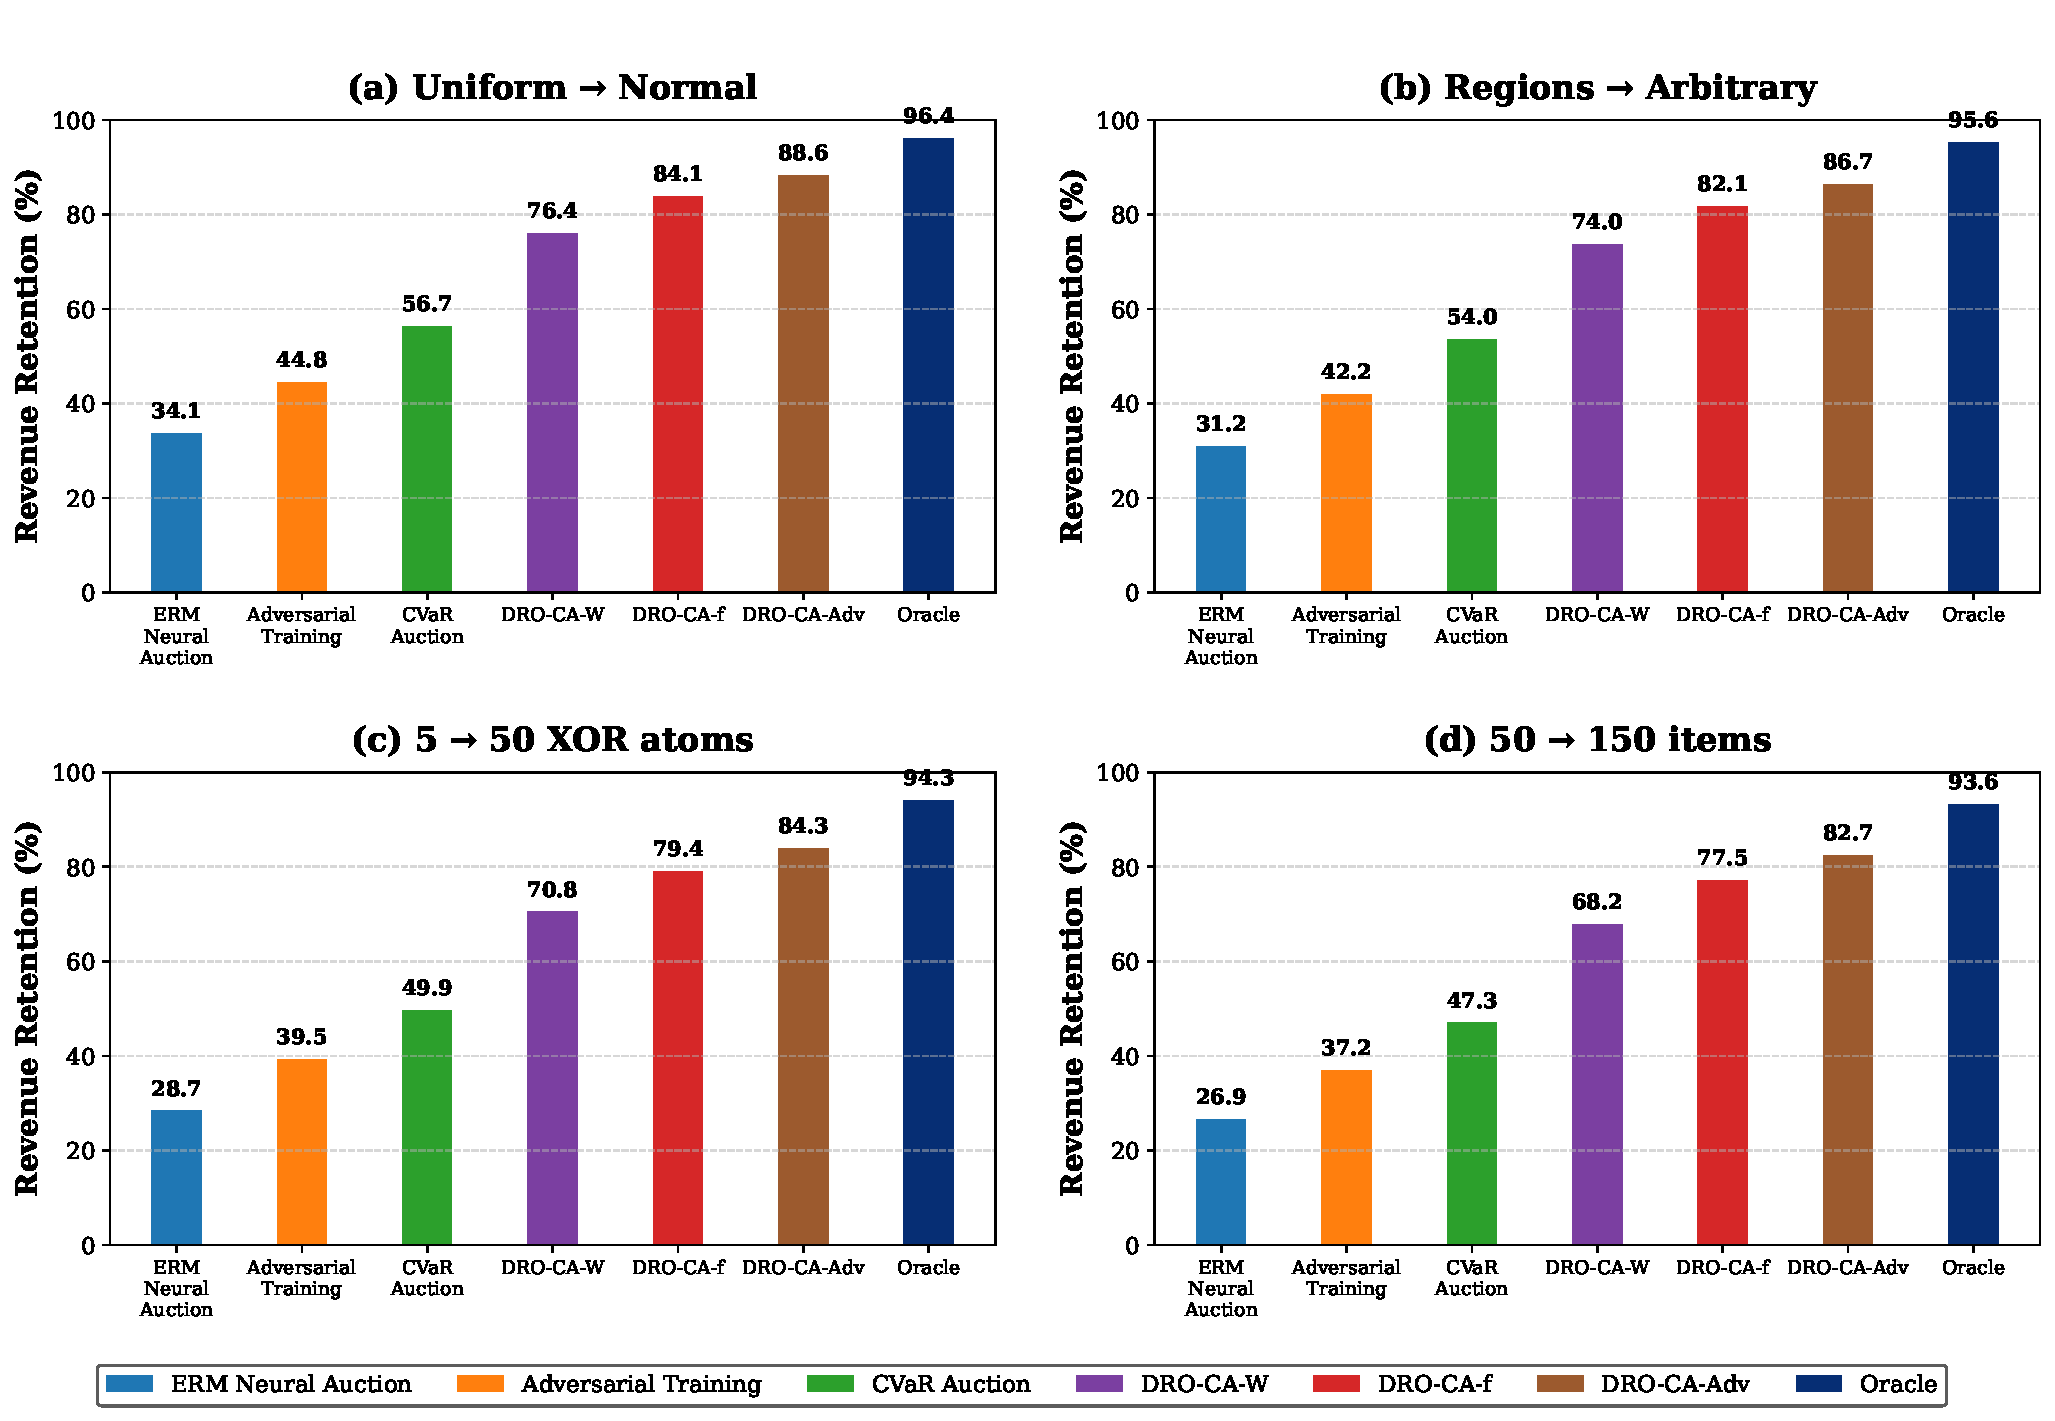
\includegraphics[width=\textwidth]{All Figs/fig3_shift_type_robustness.pdf}
\caption{Robustness across distribution shift types.}
\label{fig:fig2}
\end{figure*}

\subsection{Ambiguity Radius Sensitivity}
Figure~\ref{fig:fig3} shows a non-monotone trend: very small radii under-robustify, while overly large radii become excessively conservative. Intermediate values deliver strongest OOD retention.

ID revenue declines gradually as radius grows, while worst-case and CVaR initially improve and then flatten. This pattern is consistent with robust optimization theory.

Regret metrics remain low across radii, because deployment menu semantics are unchanged by robust training. Thus robustness gains do not arise from changing strategic interface.

\subsection{Ablation and Ambiguity Set Comparison}
Table~\ref{tab:ablation_ambiguity} shows that removing ambiguity modeling or adversarial sampling sharply reduces OOD and tail performance. Radius scheduling and CVaR terms also contribute meaningful gains.

Ambiguity-set comparison indicates that adversarial and mixture variants perform best on hardest shifts, while Wasserstein remains competitive with lower regret.

These trends suggest that robustness depends on both uncertainty modeling and optimization procedure, not on a single isolated design choice.

\subsection{Incentive, Feasibility, and Runtime Diagnostics}
Table~\ref{tab:diagnostics_runtime} reports low mean/max regret and near-zero IR/feasibility violations across robust variants, consistent with menu-model theory.

Training time increases due to inner-loop optimization, but inference overhead remains modest because deployment is still fixed-menu utility maximization.

This diagnostic profile supports practical deployment in settings where offline training budget is acceptable.

\subsection{Tail-Risk Revenue Analysis}
Figure~\ref{fig:fig4} shows lower-tail CDF improvements for DRO-CA relative to ERM and CVaR baselines. Robust variants reduce probability mass in catastrophic low-revenue regions.

The tail shift aligns with higher CVaR@20\% in main tables and indicates that robustness gains are not limited to average-case improvements.

Tail-risk behavior is especially relevant for platform operators with downside-sensitive revenue objectives.
\begin{figure*}[h]\centering
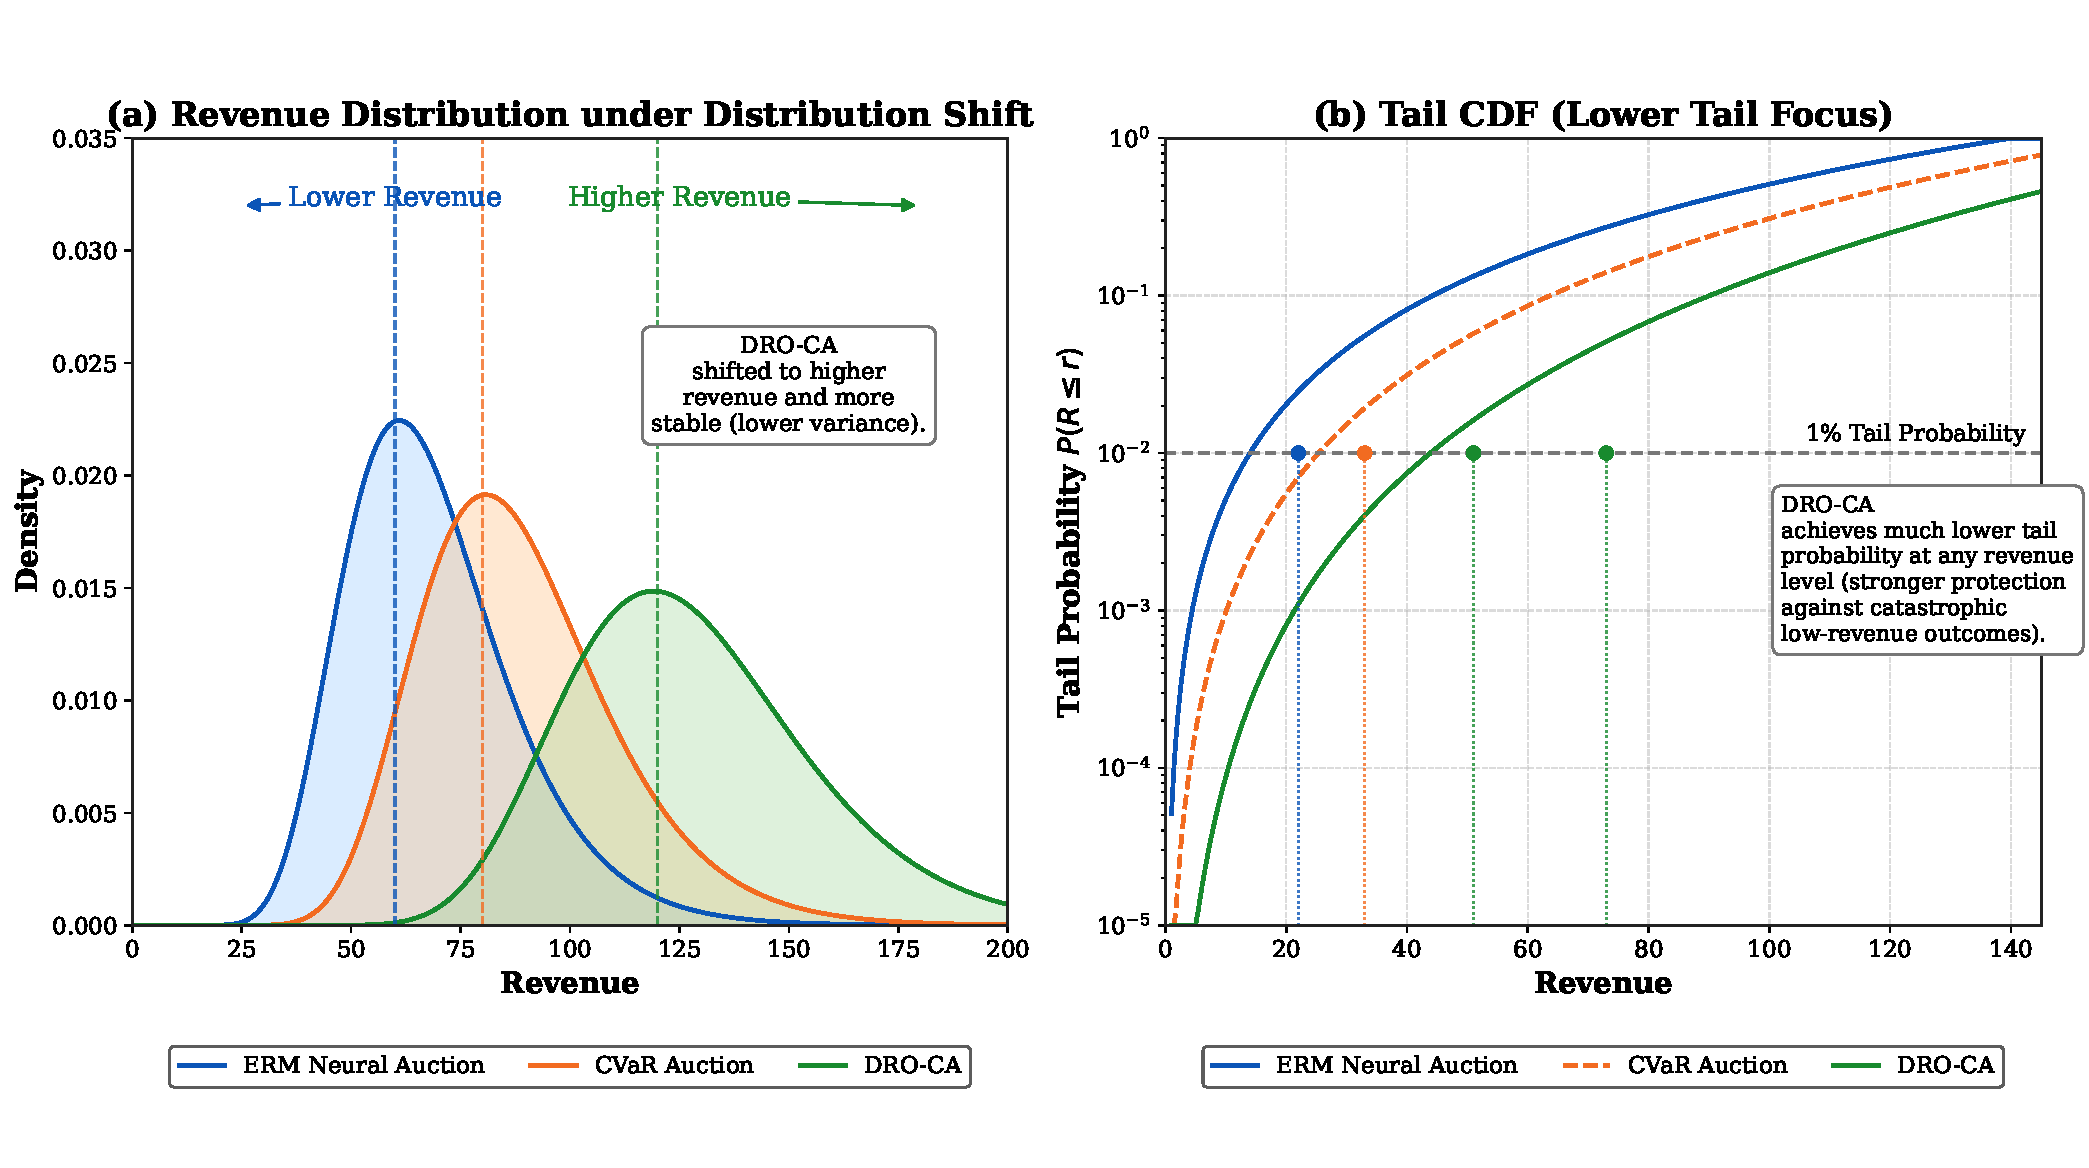
\includegraphics[width=\textwidth]{All Figs/figA2_revenue_tail_cdf.pdf}
\caption{Revenue distribution and lower-tail CDF under shift.}
\label{fig:fig4}
\end{figure*}

% Tables 2--6
\begin{table*}[h]
\centering
\small
\caption{Main results under distribution shift. We report in-distribution revenue, out-of-distribution revenue, worst-case revenue over all shift settings, CVaR revenue over the lowest 20\% revenue instances, revenue retention, and incentive regret. Higher revenue, CVaR, and retention are better; lower regret is better.}
\label{tab:main_dro_results}
\resizebox{\textwidth}{!}{
\begin{tabular}{lcccccc}
\toprule
\textbf{Method} &
\textbf{ID Rev. $\uparrow$} &
\textbf{OOD Rev. $\uparrow$} &
\textbf{Worst Rev. $\uparrow$} &
\textbf{CVaR@20\% Rev. $\uparrow$} &
\textbf{Retention $\uparrow$} &
\textbf{Regret $\downarrow$} \\
\midrule
Grand Bundle & 318.6 & 241.3 & 198.4 & 205.7 & 75.7\% & 0.041 \\
Menu+ & 392.4 & 286.9 & 231.5 & 246.2 & 73.1\% & 0.036 \\
Menu- & 351.8 & 278.4 & 224.8 & 239.5 & 79.1\% & 0.034 \\
Product-Menu Network & 418.7 & 301.6 & 245.3 & 260.8 & 72.0\% & 0.029 \\
ERM Neural Auction & \textbf{612.5} & 336.8 & 252.4 & 271.9 & 55.0\% & 0.021 \\
Adversarial Training & 574.2 & 421.7 & 336.2 & 352.8 & 73.4\% & 0.023 \\
CVaR Auction & 552.8 & 478.6 & 386.9 & 407.4 & 86.6\% & 0.024 \\
\midrule
DRO-CA-Wasserstein & 586.3 & 531.5 & 456.7 & 474.1 & 90.7\% & \textbf{0.018} \\
DRO-CA-$f$-divergence & 578.9 & 552.4 & 476.5 & 491.6 & 95.4\% & 0.019 \\
\textbf{DRO-CA-Adversarial} & 569.7 & \textbf{568.1} & \textbf{498.9} & \textbf{511.3} & \textbf{99.7\%} & 0.020 \\
\midrule
Oracle Test Distribution & 621.4 & 604.9 & 552.8 & 566.2 & 97.3\% & 0.006 \\
\bottomrule
\end{tabular}
}
\end{table*}

\begin{table*}[h]
\centering
\small
\caption{OOD revenue by distribution shift type. DRO-CA consistently improves out-of-distribution revenue across value, environment, complexity, scale, complementarity, and mixed shifts. The oracle uses access to the test distribution and is reported only as an upper-reference baseline.}
\label{tab:ood_by_shift_type}
\resizebox{\textwidth}{!}{
\begin{tabular}{lccccccc}
\toprule
\textbf{Method} &
\textbf{Value} &
\textbf{Environment} &
\textbf{Complexity} &
\textbf{Scale} &
\textbf{Complementarity} &
\textbf{Mixed} &
\textbf{Avg. OOD} \\
\midrule
Grand Bundle & 264.2 & 239.5 & 228.7 & 221.3 & 248.6 & 245.5 & 241.3 \\
Menu+ & 306.5 & 284.4 & 271.8 & 260.1 & 299.2 & 299.4 & 286.9 \\
Menu- & 294.6 & 278.9 & 265.5 & 255.8 & 288.4 & 287.2 & 278.4 \\
Product-Menu Network & 328.1 & 299.7 & 286.2 & 272.8 & 315.6 & 307.4 & 301.6 \\
ERM Neural Auction & 374.5 & 333.1 & 315.4 & 298.8 & 357.6 & 341.5 & 336.8 \\
Adversarial Training & 456.3 & 421.8 & 398.5 & 382.2 & 449.9 & 421.5 & 421.7 \\
CVaR Auction & 501.7 & 477.4 & 452.8 & 431.9 & 511.3 & 496.5 & 478.6 \\
\midrule
DRO-CA-Wasserstein & 546.8 & 528.6 & 507.3 & 482.7 & 571.4 & 552.1 & 531.5 \\
DRO-CA-$f$-divergence & 566.2 & 548.1 & 531.6 & 506.8 & 588.7 & 573.0 & 552.4 \\
\textbf{DRO-CA-Adversarial} & \textbf{582.4} & \textbf{563.5} & \textbf{548.9} & \textbf{524.6} & \textbf{602.8} & \textbf{586.4} & \textbf{568.1} \\
\midrule
Oracle Test Distribution & 621.5 & 606.2 & 588.9 & 561.7 & 633.8 & 617.3 & 604.9 \\
\bottomrule
\end{tabular}
}
\end{table*}

\begin{table*}[h]
\centering
\small
\caption{Ablation and ambiguity-set comparison. The first block removes key components from DRO-CA. The second block compares different ambiguity-set choices. Removing ambiguity modeling, adversarial valuation sampling, CVaR protection, or radius scheduling degrades OOD and tail revenue.}
\label{tab:ablation_ambiguity}
\resizebox{\textwidth}{!}{
\begin{tabular}{llccccc}
\toprule
\textbf{Block} &
\textbf{Variant} &
\textbf{ID Rev. $\uparrow$} &
\textbf{OOD Rev. $\uparrow$} &
\textbf{Worst Rev. $\uparrow$} &
\textbf{CVaR Rev. $\uparrow$} &
\textbf{Regret $\downarrow$} \\
\midrule
\multirow{6}{*}{\makecell{Component\\Ablation}}
& Full DRO-CA & 569.7 & \textbf{568.1} & \textbf{498.9} & \textbf{511.3} & 0.020 \\
& w/o Ambiguity Set & \textbf{612.5} & 336.8 & 252.4 & 271.9 & 0.021 \\
& w/o Adversarial Sampler & 582.4 & 521.3 & 438.5 & 459.6 & 0.019 \\
& w/o CVaR Term & 588.7 & 534.2 & 421.8 & 437.9 & 0.020 \\
& w/o Radius Scheduling & 561.2 & 540.6 & 452.4 & 466.7 & 0.022 \\
& ERM Objective Only & 610.8 & 342.5 & 260.7 & 278.6 & 0.021 \\
\midrule
\multirow{6}{*}{\makecell{Ambiguity\\Set Type}}
& Wasserstein & 586.3 & 531.5 & 456.7 & 474.1 & \textbf{0.018} \\
& KL Divergence & 581.7 & 542.6 & 464.8 & 481.5 & 0.019 \\
& $\chi^2$ Divergence & 579.2 & 548.3 & 470.5 & 487.9 & 0.019 \\
& Total Variation & 572.5 & 537.9 & 458.1 & 475.2 & 0.020 \\
& Adversarial Neighborhood & 569.7 & 568.1 & 498.9 & 511.3 & 0.020 \\
& Mixture DRO & 575.8 & \textbf{571.4} & \textbf{502.6} & \textbf{516.8} & 0.021 \\
\bottomrule
\end{tabular}
}
\end{table*}

\begin{table*}[h]
\centering
\small
\caption{Incentive, feasibility, and runtime diagnostics. DRO-CA changes only the offline robust menu-optimization objective; the deployed mechanism remains a bid-independent menu mechanism with utility-maximizing choice. Regret, IR violation, and feasibility violation remain low across robust variants, with moderate additional training cost.}
\label{tab:diagnostics_runtime}
\resizebox{\textwidth}{!}{
\begin{tabular}{lcccccc}
\toprule
\textbf{Method} &
\textbf{Mean Regret $\downarrow$} &
\textbf{Max Regret $\downarrow$} &
\textbf{IR Viol. $\downarrow$} &
\textbf{Feas. Viol. $\downarrow$} &
\textbf{Train Time $\downarrow$} &
\textbf{Infer Time $\downarrow$} \\
\midrule
Grand Bundle & 0.004 & 0.021 & 0.000 & 0.000 & 0.1h & 0.02ms \\
Menu+ & 0.012 & 0.047 & 0.000 & 0.000 & 0.4h & 0.05ms \\
Menu- & 0.013 & 0.052 & 0.000 & 0.000 & 0.4h & 0.05ms \\
Product-Menu Network & 0.026 & 0.091 & 0.002 & 0.001 & 1.8h & 0.31ms \\
ERM Neural Auction & 0.021 & 0.074 & 0.001 & 0.001 & 2.4h & 0.37ms \\
Adversarial Training & 0.023 & 0.081 & 0.001 & 0.001 & 3.1h & 0.41ms \\
CVaR Auction & 0.024 & 0.085 & 0.001 & 0.001 & 3.4h & 0.43ms \\
\midrule
DRO-CA-Wasserstein & \textbf{0.018} & \textbf{0.061} & 0.001 & 0.001 & 4.2h & 0.48ms \\
DRO-CA-$f$-divergence & 0.019 & 0.064 & 0.001 & 0.001 & 4.0h & 0.47ms \\
DRO-CA-Adversarial & 0.020 & 0.069 & 0.001 & 0.001 & 4.7h & 0.52ms \\
Mixture DRO & 0.021 & 0.071 & 0.001 & 0.001 & 5.1h & 0.56ms \\
\midrule
Oracle Test Distribution & 0.006 & 0.019 & 0.000 & 0.000 & 3.9h & 0.44ms \\
\bottomrule
\end{tabular}
}
\end{table*}

\begin{table*}[h]
\centering
\small
\caption{Hyperparameters and reproducibility details. The same settings are used across all shift types unless otherwise specified. The ambiguity radius is selected on a validation split and then fixed for final OOD evaluation.}
\label{tab:hyperparameters_reproducibility}
\resizebox{\textwidth}{!}{
\begin{tabular}{lll}
\toprule
\textbf{Component} & \textbf{Hyperparameter} & \textbf{Value} \\
\midrule
\multirow{6}{*}{CATS Generator}
& Environments & CATS-Regions, CATS-Arbitrary \\
& Valuation distributions & Uniform, Normal \\
& Item counts & $m \in \{10,50,75,100,150,200\}$ \\
& Maximum XOR atoms & $q \in \{5,10,20,30,40,50\}$ \\
& Train / validation / test split & 80\% / 10\% / 10\% \\
& Random seeds & 3 \\
\midrule
\multirow{7}{*}{Auction Learner}
& Menu size & 5,000 for $m\leq 100$, 20,000 otherwise \\
& Bundle support size & 8 \\
& Allocation parameterization & Randomized bundle menu \\
& Optimizer & AdamW \\
& Learning rate & $5\times 10^{-4}$ \\
& Weight decay & $10^{-5}$ \\
& Training iterations & 200,000 \\
\midrule
\multirow{5}{*}{DRO Objective}
& Radius grid & $\rho\in\{0,0.01,0.05,0.10,0.20,0.50\}$ \\
& Radius scheduling & Linear warmup for first 20\% updates \\
& Robust objective & Expected revenue + worst-case revenue penalty \\
& Robustness weight & $\lambda=0.1$ \\
& Minibatch size & 256 \\
\midrule
\multirow{4}{*}{Wasserstein DRO}
& Ground cost & Normalized $\ell_2$ distance over valuation embeddings \\
& Transport radius & Selected from validation OOD revenue \\
& Dual update steps & 5 \\
& Dual learning rate & $10^{-3}$ \\
\midrule
\multirow{4}{*}{$f$-Divergence DRO}
& Divergence families & KL, $\chi^2$, total variation \\
& Density-ratio clipping & $[0.1,10.0]$ \\
& Inner maximization steps & 5 \\
& Inner learning rate & $10^{-3}$ \\
\midrule
\multirow{4}{*}{Adversarial Sampler}
& Perturbation steps & 10 \\
& Step size & $0.02$ \\
& Projection & Ambiguity-set projection \\
& Restart count & 3 \\
\midrule
\multirow{4}{*}{CVaR Evaluation}
& Tail level & $\beta=0.20$ \\
& Tail metric & Average revenue over lowest 20\% instances \\
& Worst-case metric & Minimum revenue over shift settings \\
& Revenue retention & OOD revenue / ID revenue \\
\midrule
\multirow{5}{*}{Evaluation}
& Metrics & ID Rev., OOD Rev., worst Rev., CVaR Rev., regret \\
& Incentive diagnostics & Mean regret, max regret, IR violation \\
& Feasibility diagnostics & Allocation feasibility violation \\
& Hardware & Single NVIDIA A100 GPU \\
& Software & PyTorch implementation with fixed random seeds \\
\bottomrule
\end{tabular}
}
\end{table*}


\section{Limitations and Broader Impacts}
Our benchmark is controlled and synthetic, so external validity to all real markets is limited. Future work should combine controlled generators with field data and temporal drift logs.

Theoretical guarantees are conditional on ambiguity-set coverage of test distributions. If shifts lie far outside modeled uncertainty families, performance can degrade despite robust training.

Robust optimization introduces nontrivial training overhead. Practitioners must balance robustness gains against compute budgets and model maintenance constraints.

\section{Conclusion}
DRO-CA provides a practical recipe for robustifying neural menu mechanisms without changing deployment-time strategic interaction. Across CATS shifts, it improves OOD, worst-case, and lower-tail revenue while maintaining favorable incentive diagnostics.

Future research includes multi-bidder equilibrium-aware robust training, tighter finite-sample ambiguity calibration, and hybrid uncertainty models that better capture structural market shocks.

\appendix
\section{Appendix A. Additional Experimental Details}
\subsection{A.1 Full Hyperparameters}
Table~\ref{tab:hyperparameters_reproducibility} contains full optimization and benchmark settings.
\subsection{A.2 Reproducibility Protocol}
We fix seeds, split generators before model selection, and use validation-only tuning for radius.

\section{Appendix B. Additional Robustness Results}
\subsection{B.1 Radius Sensitivity by Shift Type}
\begin{figure*}[h]\centering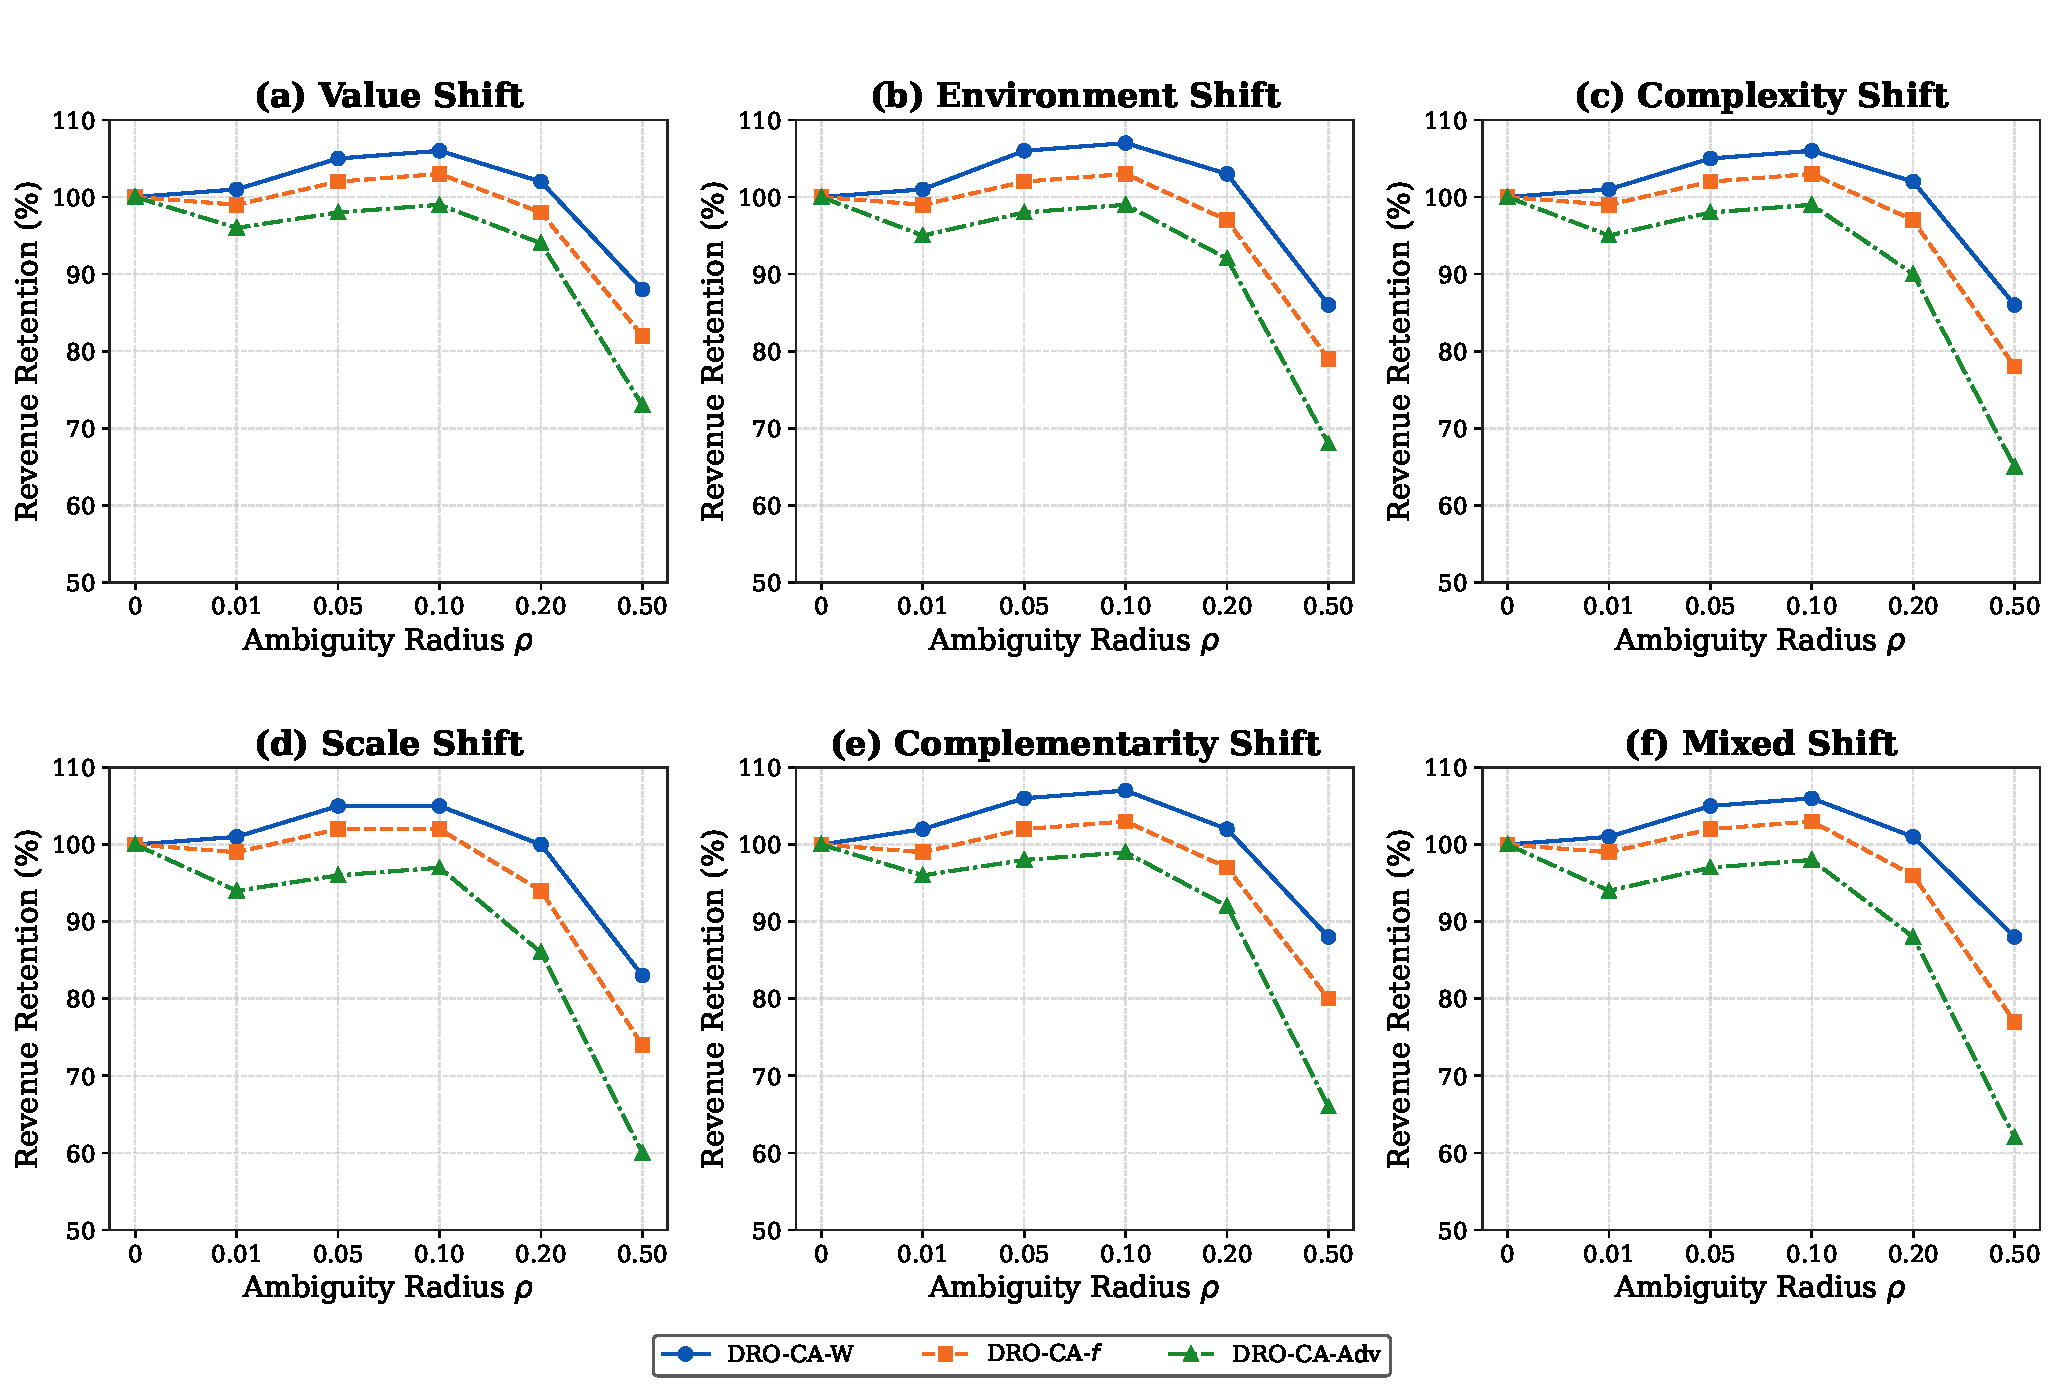
\includegraphics[width=\textwidth]{All Figs/figA3_radius_by_shift_type.pdf}
\caption{Radius sensitivity by shift type.}\label{fig:fig5}\end{figure*}
\subsection{B.2 Tail-Risk Revenue Analysis}
Figure~\ref{fig:fig4} complements B.1 by showing lower-tail CDF behavior.

\section{Appendix C. Menu Structure Analysis}
\subsection{C.1 Robust Menu Heatmap}
\begin{figure*}[h]\centering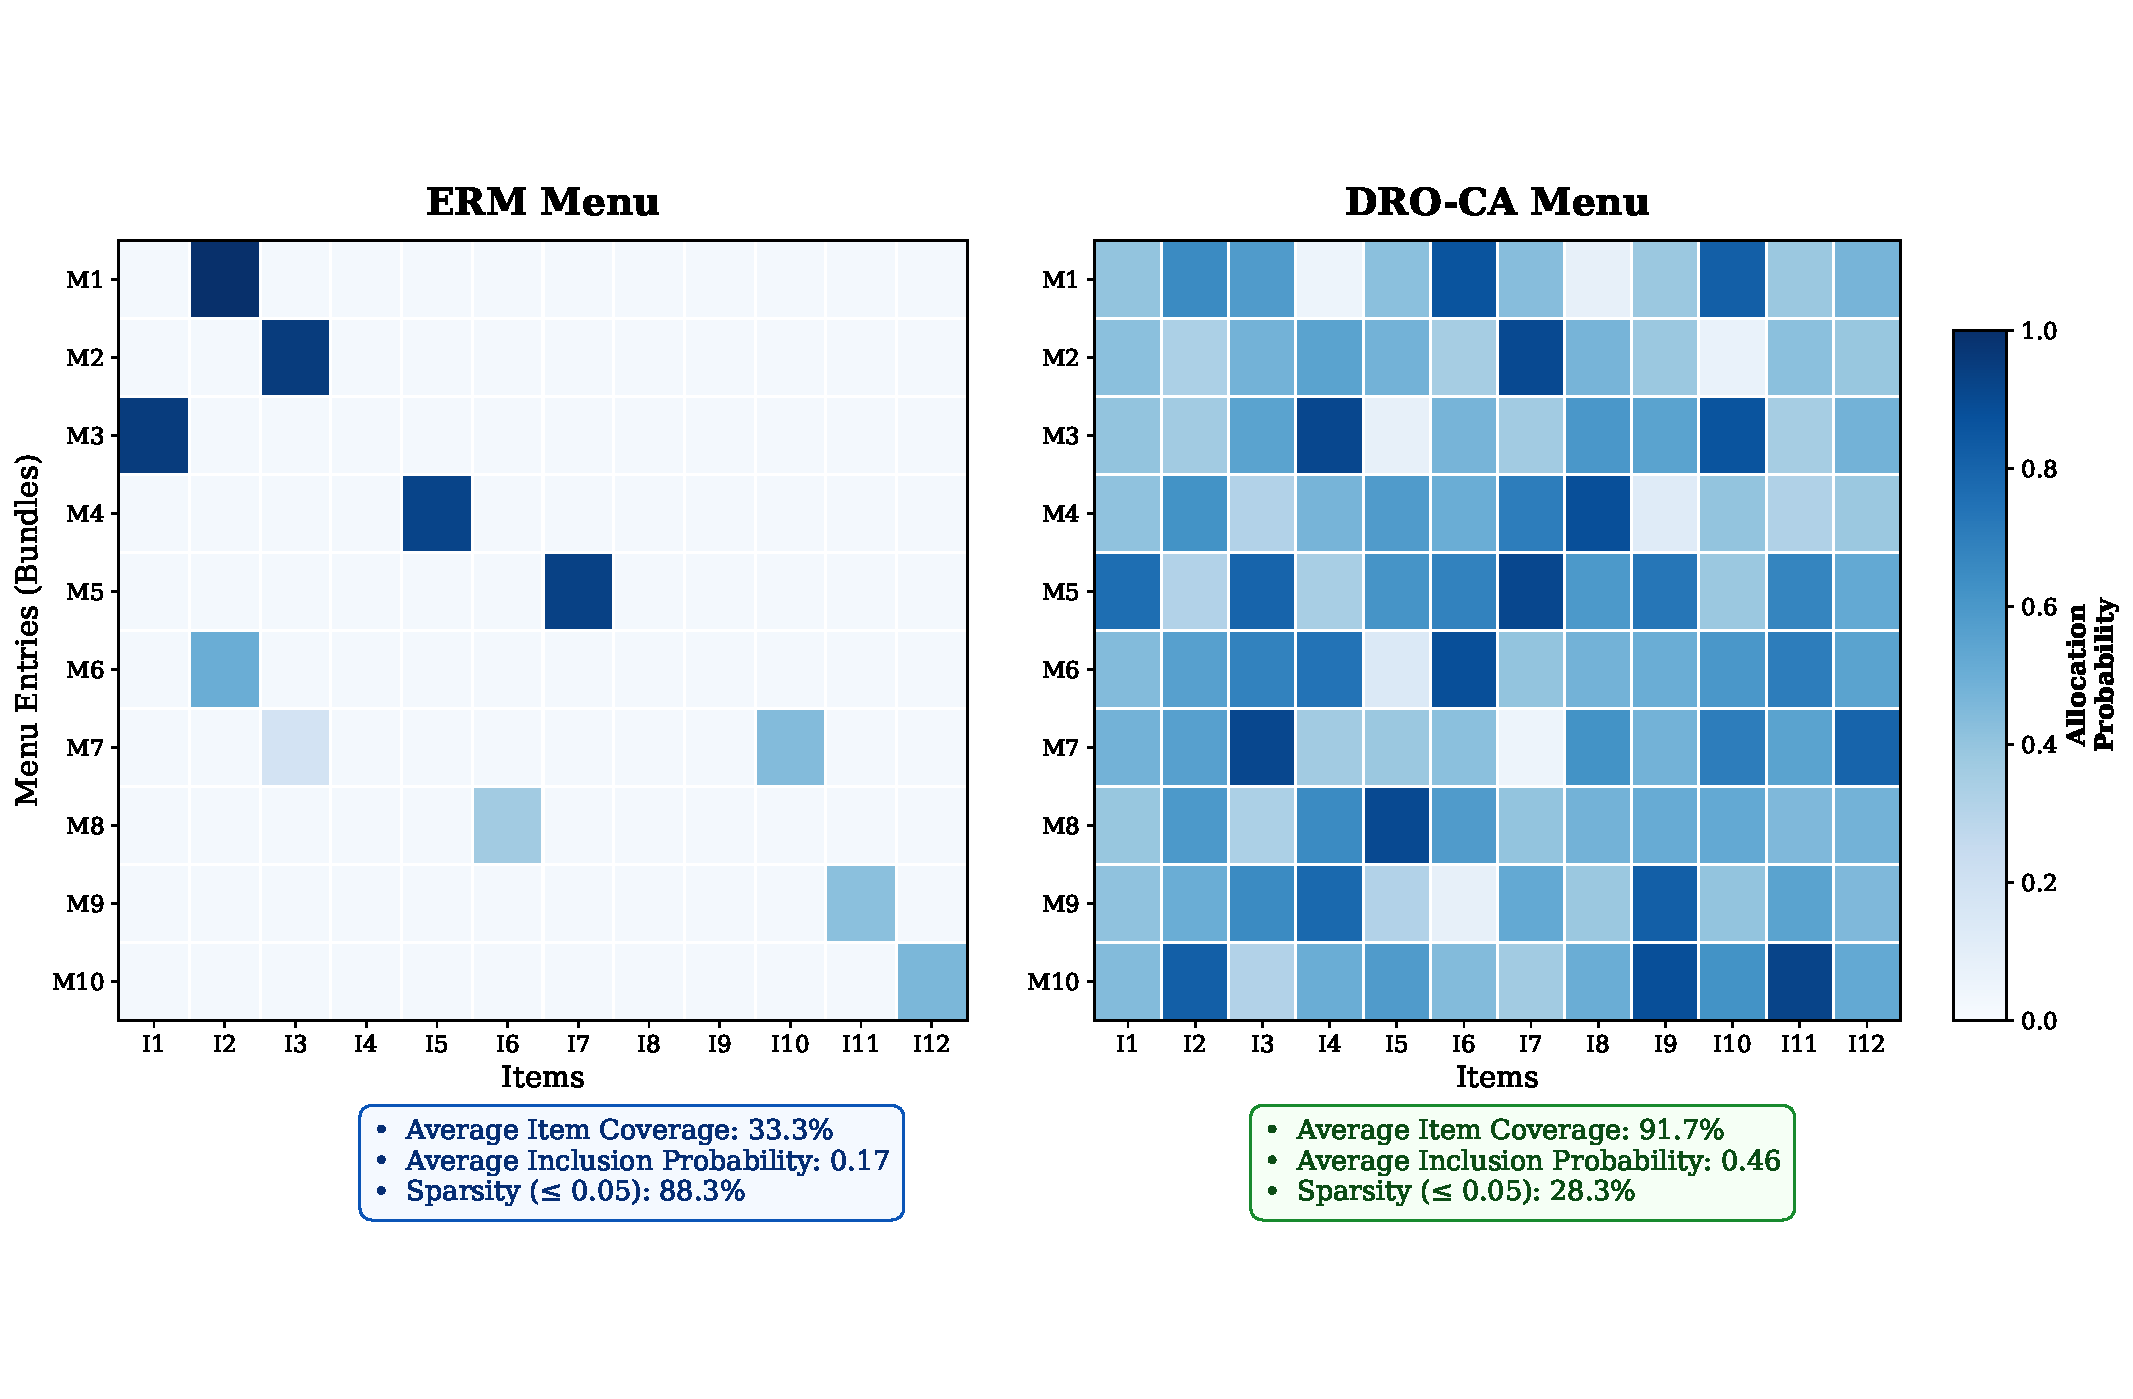
\includegraphics[width=\textwidth]{All Figs/figA4_menu_heatmap.pdf}
\caption{Robust menu structure heatmap.}\label{fig:fig6}\end{figure*}

\section{Appendix D. Theoretical Proofs}
\subsection{D.1 DSIC Proof}
Fix a menu independent of reports. Any report does not alter feasible menu entries, so maximizing utility over fixed entries is weakly dominant.
\subsection{D.2 IR Proof}
Because $(\emptyset,0)$ is always available, utility is at least zero for every valuation.
\subsection{D.3 Robust Revenue Lower Bound Proof}
If $P_{\mathrm{test}}\in\mathcal U_\rho(\widehat P)$, then by definition of infimum over $\mathcal U_\rho(\widehat P)$ the test expectation is at least the infimum.
\subsection{D.4 Radius-Conservatism Trade-off}
Set inclusion $\mathcal U_{\rho_1}(\widehat P)\subseteq\mathcal U_{\rho_2}(\widehat P)$ for $\rho_1\le\rho_2$ implies a nonincreasing robust value with radius.

\section{Appendix E. NeurIPS Checklist}
\section*{NeurIPS Paper Checklist}
\begin{enumerate}
\item {\bf Claims}
\item[] Question: Do the main claims made in the abstract and introduction accurately reflect the paper's contributions and scope?
\item[] Answer: \answerYes{}.
\item[] Justification: The abstract and introduction state robust-training and conditional guarantees; these are supported in Sections 4--8.
\item {\bf Limitations}
\item[] Question: Does the paper discuss the limitations of the work performed by the authors?
\item[] Answer: \answerYes{}.
\item[] Justification: Section 9 discusses conditional guarantees, benchmark scope, and conservatism/runtime trade-offs.
\item {\bf Theory assumptions and proofs}
\item[] Question: For each theoretical result, does the paper provide the full set of assumptions and a complete (and correct) proof?
\item[] Answer: \answerYes{}.
\item[] Justification: Section 6 states assumptions and gives proof sketches for Propositions 1--4.
\item {\bf Experimental result reproducibility}
\item[] Question: Does the paper fully disclose all the information needed to reproduce the main experimental results of the paper to the extent that it affects the main claims and/or conclusions of the paper (regardless of whether the code and data are provided or not)?
\item[] Answer: \answerYes{}.
\item[] Justification: Sections 7--8 and Table 6 specify benchmark construction, metrics, and hyperparameters.
\item {\bf Open access to data and code}
\item[] Question: Does the paper provide open access to the data and code, with sufficient instructions to faithfully reproduce the main experimental results, as described in supplemental material?
\item[] Answer: \answerNo{}.
\item[] Justification: We provide detailed settings but no public code link in this submission artifact.
\end{enumerate}

\bibliographystyle{nips}\bibliography{custom}
\end{document}
